\subsection{Model and Parameter}
\vspace{50pt}
\begin{figure}[H]
    \setlength{\abovecaptionskip}{50pt} 
    \centering
    \resizebox{90mm}{!}{\includegraphics{dia/model.eps}}
    \caption{Static Traffic Model}
    \label{fig:model}
\end{figure}

As figure \ref{fig:model} show, this is our wireless hoc network topo. And the key parameter of model show in table \ref{tab:para}:


\begin{table}[H]
    \centering
    \setlength{\extrarowheight}{2mm}
    \addtolength{\tabcolsep}{3mm}
    \begin{tabular}{ | l | r@{.}l | }
        \hline 
        \backslashbox{Parameter}{Value} & \multicolumn{2}{c|}{Value}  \\
        \hline
        CSThresh\_ & 5&00522e-12 \\
        \hline
        RXThresh\_ & 2&42253e-11\\
        \hline
        Pt\_ & 0&000935073 \\
        \hline
        freq\_ & 2&472e9 \\
        \hline
    \end{tabular}
    \caption{Key Parameter of model}
    \label{tab:para}
\end{table}

How to determine these parameter. We know \verb|RXThresh_| is the communication range between two nodes. \verb|CSThresh_| is the carrier sense range. These two parameter is key important factor that affect communication. In TwoRayGround model. \verb|Pr| is:

$$ Pr ~ = ~  \frac{Pt*Gt*Gr*\lambda^2}{\left(4*pi*d\right)^2*L} $$

and \verb|d| is the communication range. The rest parameter will keep the default value as them in \verb|ns-2| except \verb|Pt|. \verb|Pt| is the transmit power and interrelated with \verb|d| as:

$$ Pt ~ = ~ 7.21505664 * d^4 * e^{-11}$$ 

when $d=250$, $Pt=0.28183815$. In our model, $d=60$, so $Pt=0.000935073$.
So we can determine the \verb|CSThresh_| and \verb|RXThresh_| with \texttt{threshold.cc} tool. Just like:

\begin{verbatim}
./threshold -Pt 0.000935073 
            -fr 2.472e9 
            -m TwoRayGround 60
\end{verbatim}

\verb|RXThresh_| is assigned to this command ouput value, that is $2.42253e^{-11}$. In \verb|ns-2|, Carrier sense range is communication range 2.2 times. So the carrier range is 132. Hence:

\begin{verbatim}
./threshold -Pt 0.000935073 
            -fr 2.472e9 
            -m TwoRayGround 132 
\end{verbatim}

And $CSThresh\_=5.00522e^{-12}$. 

\begin{table}[H]
    \centering
    \setlength{\extrarowheight}{2mm}
    \addtolength{\tabcolsep}{3mm}
    \begin{tabular}{ | l | r | }
        \hline 
        \backslashbox{Parameter}{Value} & Value  \\
        \hline
        CWMin\_ & 31 \\
        \hline
        CWMax\_ & 1023 \\
        \hline
        SlotTime\_ & 0.000020 \\
        \hline
        SIFS\_ & 0.000010 \\
        \hline
        PreambleLength\_ & 144 \\
        \hline
        PLCPHeaderLength\_ & 48 \\
        \hline
        PLCPDataRate\_ & 11.0e6 \\
        \hline
        dataRate\_ & 11.0e6 \\
        \hline
        basicRate\_ & 1.0e6 \\
        \hline
    \end{tabular}
    \caption{802.11b Standard Parameter}
    \label{tab:80211}
\end{table}

The table \ref{tab:80211} show the key parameter of \verb|802.11b| standard. In this table, I just list the parameter that compare with \verb|802.11| is different.

\newpage
\subsection{Performance Analysis}
\subsubsection{Delay Compare}
\begin{figure}[H]
    \centering
    \begin{tabular}{l r}
        \resizebox{60mm}{!}{\includegraphics{eps/scenario_1/udp/ad_delay_bw.eps}} &
        \resizebox{60mm}{!}{\includegraphics{eps/scenario_1/udp/hi_delay_bw.eps}} \\
        \multicolumn{2}{c}{\resizebox{60mm}{!}{\includegraphics{eps/scenario_1/udp/lo_delay_bw.eps}}} 
    \end{tabular}
    \caption{Delay Compare}
    \label{fig:delay_1}
\end{figure}


\begin{table}[H]
    \centering
    \setlength{\extrarowheight}{2mm}
    \addtolength{\tabcolsep}{3mm}
    \begin{tabular}{c c c}
        \hline \hline
        &  Avg\myfootnotemark & Stdev\myfootnotemark \\
        \hline
        AD & 0.285798 & 0.073276 \\
        HI & 0.302772 & 0.058543 \\
        LO & 0.007705 & 0.003792 \\
        \hline
    \end{tabular}
    \caption{Delay Compare}
    \label{tab:delay_1}
\end{table}
\myfootnotetext{Avg is the abbreviation of the Average}
\myfootnotetext{Stdev is the abbreviation of the Standard deviation}

Because of the total packet is too much so that it is not a good idea to plot every packet end-to-end to the figure. I divide the packet to one hundred batch by adjusting the number of packet of each batch. Not only make the figure clear. But also can describe the trends of vary accurately. This approach also used in the remaining figure. 

In the top-left, that is adaptive rate case. The highest rate case resides on the top-right. The third figure is the lowest rate case. This location arrangement will keep consistent in entire report. 

As figure \ref{fig:delay_1} and table \ref{tab:delay_1} illustrated. Highest rate leading the highest delay and the delay of lowest rate is the minimum. Adaptive rate between them. Note that the \verb|Stdev| tell us that the jitter of delay. Since adjust delivery rate based on the loss ratio. It result in the maximum delay jitter. 

\subsubsection{Delay Jitter Compare}
\begin{figure}[H]
    \centering
    \begin{tabular}{l r}
        \resizebox{60mm}{!}{\includegraphics{eps/scenario_1/udp/ad_jitter_bw.eps}} &
        \resizebox{60mm}{!}{\includegraphics{eps/scenario_1/udp/hi_jitter_bw.eps}} \\
        \multicolumn{2}{c}{\resizebox{60mm}{!}{\includegraphics{eps/scenario_1/udp/lo_jitter_bw.eps}}} 
    \end{tabular}
    \caption{Delay jitter Compare}
\end{figure}

Define \verb|jitter| as:

$$jitter=\frac{delay_{2}-delay_{1}}{pkt\_id_{2}-pkt\_id_{1}}$$

Intuitively, Highest rate case jitter mostly above zero. Lowest rate case jitter mostly below zero. By contrast, Adaptive rate case jitter around zero. This explain why the standard deviation of delay of adaptive rate case is maximum. 

Why the delay of highest rate case is the maximum value among three case? 
As we know, end-to-end delay \verb|T| is equal to:

$$T=W+S$$

\verb|W| is queuing time and \verb|S| is transmission time. Because of the other affective factor is same, We can simple assume the transmission time is same to three case. Hence we just need to think of how the delivery rate influence the queuing time \verb|W|. Basically, the higher deliverate, the easier it is to casuse congestion and the higher queuing time. So it explain why \verb|HI| rate case with highest delay time and mostly delay jitter above zero.          


\subsubsection{Throughput Compare}
\begin{figure}[H]
    \centering
    \resizebox{90mm}{!}{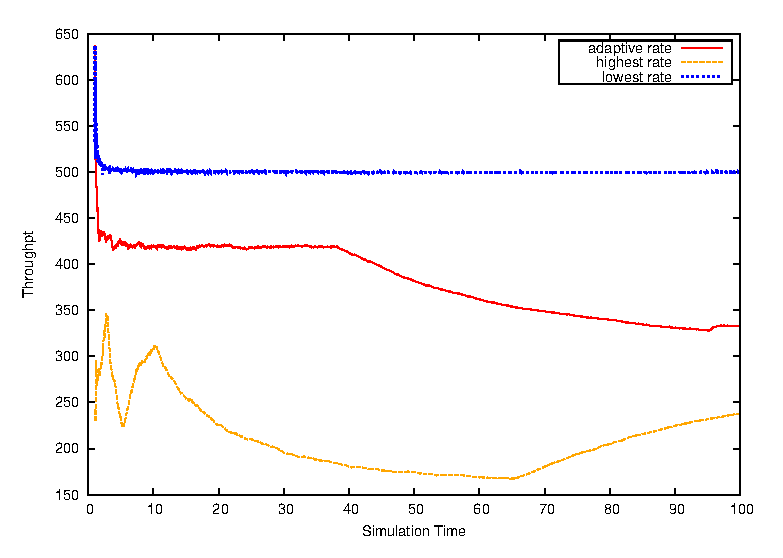
\includegraphics{eps/scenario_1/udp/throughput_bw.eps}}
    \caption{Throughput Compare}
\end{figure}

\begin{figure}[H]
    \centering
    \resizebox{90mm}{!}{\includegraphics{eps/scenario_1/udp/rate_bw.eps}}
    \caption{Adaptive Rate During Simulation Time}
\end{figure}

\begin{table}[H]
    \centering
    \setlength{\extrarowheight}{2mm}
    \addtolength{\tabcolsep}{3mm}
    \begin{tabular}{c c r@{.}l}
        \hline \hline
        &  Avg & \multicolumn{2}{c}{Stdev} \\
        \hline
        AD & 811.203610 & 21&317470 \\
        HI & 996.501545 & 39&579208 \\
        LO & 306.456949 & 6&583978 \\
        \hline
    \end{tabular}
    \caption{Throughput Compare}
\end{table}

We can find the throughput of AD case keep a stable value even thought the delivery rate adjust with the loss ratio. But also the standard deviation of throughput of AD case is smaller than HI case. The throughput curve of AD case is not far away from HI case. 

The figure also indicate that the three case get the highest throughput in the initial stage. After this stage, the throughput will keep approximate constant. That is said that network has a capacity. 

We can simply conclude that the higher delivery rate, we can get the higher throughput from this figure. However, network has a capacity. So if the delivery rate reach the congestion collapse. This conclusion would be not correct. 

\subsubsection{Loss Rate Compare}
\begin{table}[H]
    \centering
    \setlength{\extrarowheight}{2mm}
    \addtolength{\tabcolsep}{3mm}
    \begin{tabular}{c c c c}
        \hline \hline
        &  Send Packets & Receive Packets & Loss Rate \\
        \hline
        AD & 10682 & 9926 & 0.070773 \\
        HI & 12825 & 11675 & 0.089669 \\
        LO & 4127 & 3709 & 0.101284 \\
        \hline
    \end{tabular}
    \caption{Loss Compare}
\end{table}
Because, this streams multimedia application adapts the delivery rate based on loss ratio. So the AD case get the lowest loss ratio. But counterintuitive, we found that the lowest delivery rate reach the highest loss ratio. The reason for this problem may be the \verb|CBR| application between \verb|node_1| and \verb|node_4|. This QOAS application content the resource with CBR. Because of the lowest delivery rate, it will fail almost time. So the loss ratio of \verb|LO| case is maximum. 


\subsubsection{PSNR Compare}
\begin{figure}[H]
    \centering
    \begin{tabular}{l r}
        \resizebox{60mm}{!}{\includegraphics{eps/scenario_1/udp/ad_psnr_bw.eps}} &
        \resizebox{60mm}{!}{\includegraphics{eps/scenario_1/udp/hi_psnr_bw.eps}} \\
        \multicolumn{2}{c}{\resizebox{60mm}{!}{\includegraphics{eps/scenario_1/udp/lo_psnr_bw.eps}}} 
    \end{tabular}
    \caption{PSNR Compare}
\end{figure}

\begin{table}[H]
    \centering
    \setlength{\extrarowheight}{2mm}
    \addtolength{\tabcolsep}{3mm}
    \begin{tabular}{c c r@{.}l}
        \hline \hline
        &  Avg & \multicolumn{2}{c}{Stdev} \\
        \hline
        AD & 49.662991 & 30&957876 \\
        HI & 24.298941 & 17&519222 \\
        LO & 99.901597 & 3&353683 \\
        \hline
    \end{tabular}
    \caption{PSNR Compare}
\end{table}

\verb|PSNR| is estimated according to the formula present below:

$$ PSNR ~ = ~ 20 \cdot log_{10} \left( \frac{MAX\_Bitrate}{\sqrt{{\left(EXP\_Thr-CRT\_Thr\right)}^2}} \right) $$

Basically, The higher \verb|PSNR|, the communication quality reach higher. We can found that the \verb|PSNR| of \verb|AD| jitter sharply. The highest \verb|PSNR| archive when the delivery rate is lowest. But \verb|PSNR| of the \verb|AD| case should be enough. 

\subsubsection{Summary}
\begin{table}[H]
    \centering
    %\setlength{\extrarowheight}{2mm}
    %\addtolength{\tabcolsep}{3mm}
     \begin{tabular}{|c|c|c|c|c|}
        \hline 
        \backslashbox{Case}{Performance} & $\overline{Delay}$ & $\overline{Throughput}$ & $\overline{Loss}$ & $\overline{PSNR}$ \\
        \hline
        AD & \textcircled{2}& \textcircled{2} & \textcircled{1} & \textcircled{2}\\
        \hline
        HI & \textcircled{3}& \textcircled{1} & \textcircled{2} & \textcircled{3}\\
        \hline
        LO & \textcircled{1}& \textcircled{3} & \textcircled{3} & \textcircled{1}\\
        \hline
    \end{tabular}
    \caption{Best Performance Sorting}
\end{table}

To sum up, I give a rank table between three case. \textcircled{1} mean the best choice in corresponding performance. \textcircled{3} mean the worst choice. Comprehensive consideration of various factors, I think the \verb|QOAS_AD| is the best solution among three case.
